\documentclass[12pt, a4paper, notitlepage]{scrreprt}
        \usepackage
        {amssymb}
        \usepackage
        {amsmath}
        \usepackage
        {verbatim, fontenc}
        \usepackage
        {tabulary, float}
        \usepackage[locale = DE, space - before - unit = true, per - mode = symbol]{siunitx}
        \usepackage
        {icomma}
        \usepackage
        {booktabs, multirow}
        \usepackage[breaklinks = true, colorlinks = true, linkcolor = blue, urlcolor = blue, citecolor = blue]{hyperref}
        \usepackage[autostyle]
        {csquotes}
        \usepackage
        {wrapfig}
        \usepackage[format = plain]{caption}
        \usepackage
        {eurosym}
        \usepackage[ngerman]
        {babel}
        \usepackage[backend = biber, style = numeric, sorting = none]{biblatex}
        \usepackage
        {gensymb}
        \DeclareMathOperator
        {\sinc}{sinc}
        \DeclareSIUnit
        {\dBm}{dBm}
        \DeclareSIUnit[per - mode = reciprocal]\WN
        {\per\centi\meter}
        \usepackage
        {chngcntr}
        \usepackage
        {graphicx, subcaption}
        \usepackage[normalem]
        {ulem}
        \useunder
        {\uline}{\ul}{}
        \usepackage[table, xcdraw]
        {xcolor}
        \title
        {\centering Solarpotential Agrivoltaics Bericht}
        \author
        {Luis Reitmeier\thanks {\href {mailto: reitmeierluis@icloud.com} {reitmeierluis@icloud.com}}}
        \date{\today}

        \begin
        {document}

        \counterwithout
        {footnote}
        {chapter}

        \maketitle

        \vfill
        \section * {Abstract}
        The following report is a detailed analysis of the solar potential of the coordinates from North 47.29 to 47.29 and east 11.47 to 11.47 with a total area of 0.85 ha
        . Figures and calculations are presented to give a comprehensive overview of the solar potential and economic potential of the area.
        
        \pagenumbering
        {arabic}
        \newpage

        \chapter
        {Assumptions}
        
        In order to simplify the calculations for a first estimation, the following assumptions were made. These assumptions are based on 
        the current market conditions in Tyrol.
        
        \begin{itemize}
        \item 30 percent of the area is covered with solar panels
        \item The solar panels have an peak power of 300 W/m²
        \item On a given day, the solar panels can use about 30 percent of the sunhours for energy production with peak power
        \item The energy selling price is 10ct/kWh. This price is assumed to increase by 3% annually.
        \item The initial build cost of the solar farm is 1€/Watt
        
        \end{itemize}
        
        With these assumptions, we can create a generall overview of the economic potential of the solar farm.
        In coming reports, the use of energy storage and the impact of government subsidies will be included in the calculations.
        Energy storage is especially interesting for on side use and for using higher prices when selling to the grid.

        \begin{figure}
        \centering
        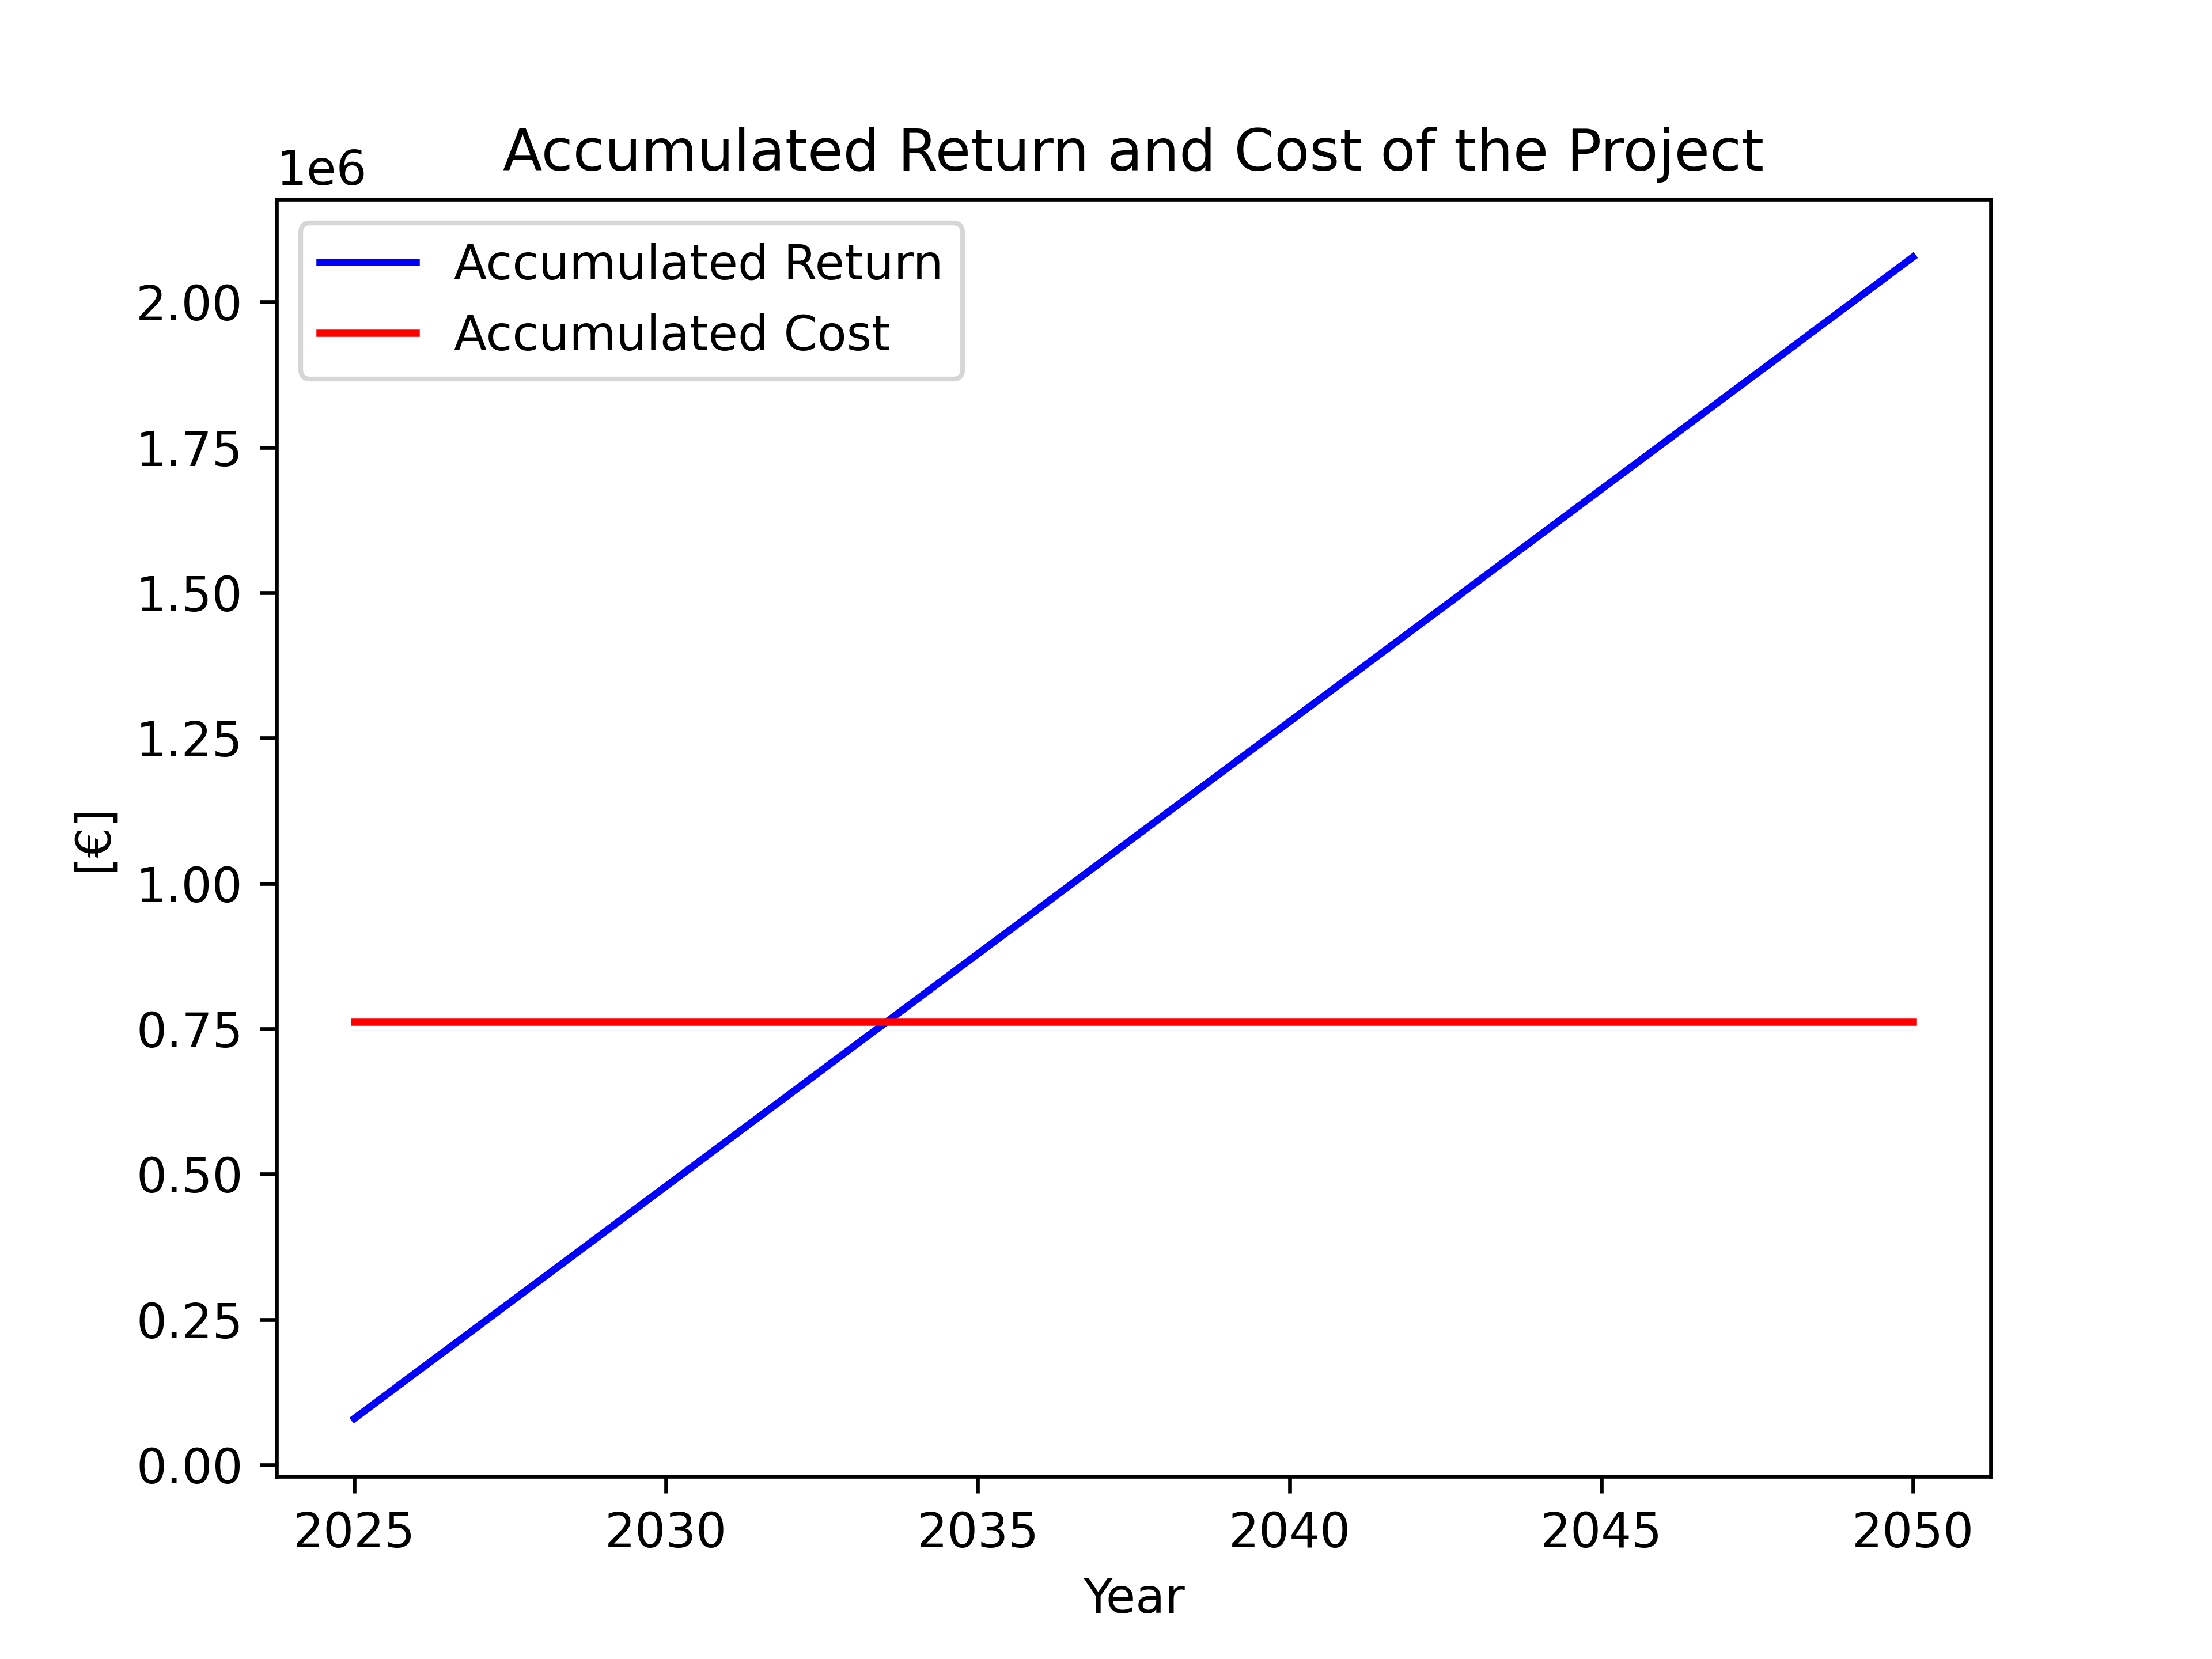
\includegraphics[scale = 0.7]{images/Akkumulierter_Ertrag.png}
        \caption {The graphic shows the accumulated cost and return of the project on the given coordinates on a timeframe of 25 years, from 2025 to 2050. The red line indicates the initial build cost,
        including planning, material and construction.}\label{Projektkosten}
        \end
        {figure}


        \begin{figure}
        \centering
        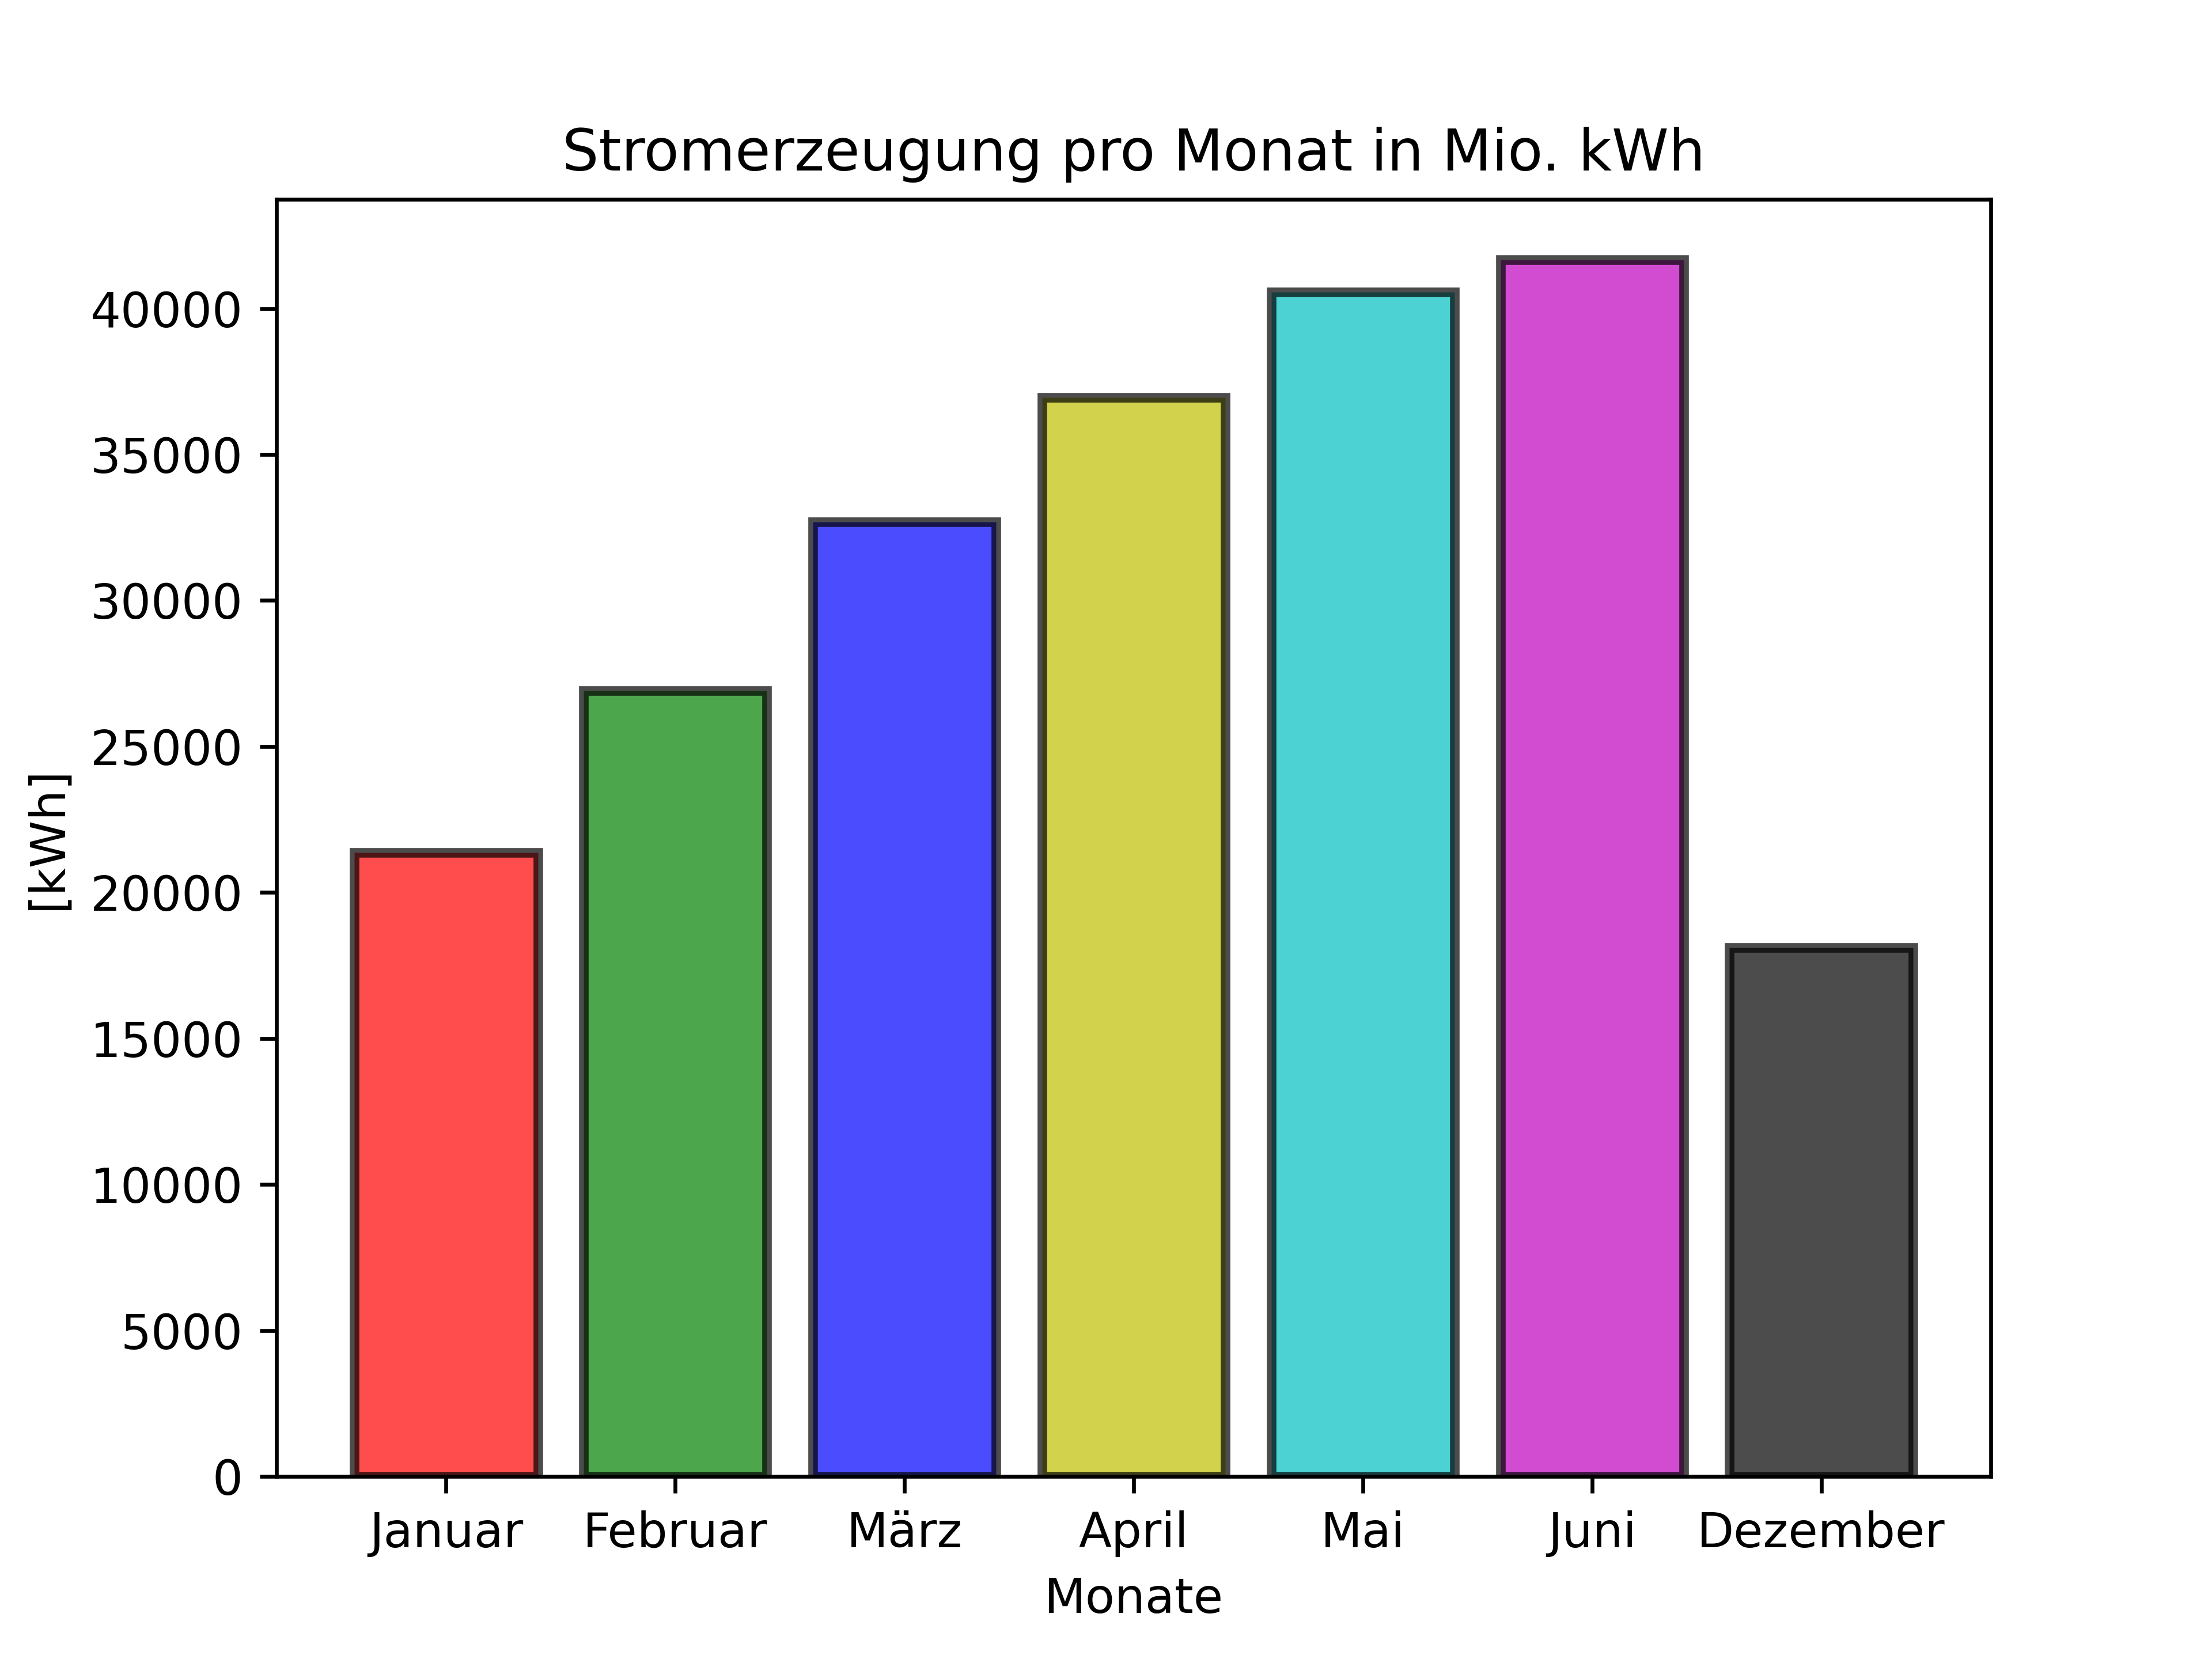
\includegraphics[scale = 0.7]{images/Stromerzeugung_pro_Monat.png}
        \caption{This graphic shows the monthly energy production of the solar farm on the given coordinates. The energy production is measured in kWh and is calculated for a timeframe of 30 days.}\label{Stromerzeugung}
        \label{Stromerzeugung}
        \end
        {figure}



        \end
        {document}